%%%%%%%%%%%%%%%%%%%%%%%%%%%%%%%% 
\section{Beam Line Measurements} 
\label{sec:detectors-nd-ref-blm}

This chapter outlines the DUNE strategy for measurements of secondary
beam particles in the region behind the beam absorber. 
Those measurements are designed to provide constraints 
on the neutrino flux at the near and far
detectors, and data on the pulse-to-pulse variation
of the beam for beam diagnostic purposes. A description of equipment
for monitoring the proton beam's interaction with the proton target
can be found in Volume 2: The Beamline at the Near Site. \fixme{The Physics Volume, Volume 2 does not have a ``Beamline at the near site chapter''}

The measurements and apparatus described in this chapter fall into
the category of equipment designed specifically for DUNE to
detect muons exiting the decay tunnel. 

\subsection{Design Considerations}
\label{subsec:detectors-nd-blm-design}

The requirements for the beamline measurements, as discussed in the
NDC requirements documentation\cite{nd_requirements_doc}, \fixme{old
LBNE reference} are intimately related to how well the neutrino flux
must be known.
%Given that DUNE does not have the luxury to construct identical 
%Near and Far Detectors, a near-far comparison is more complicated than it was in
%the MINOS experiment~\cite{gnumi-validation}, for example.   
While external hadron-production measurements can place strong 
constraints on the pion and kaon production in the target, they do not 
provide any confirmation of the simulation of other key features, such 
as the horn focusing, secondary interactions, and the 
pion scattering and absorption in the air-filled decay volume. 

In addition to the external measurements, covered in
Section~\ref{sec:detectors-nd-ref-hadron}, that confirm the
simulation of the thick target, horn material, decay tunnel and
absorber, it is desirable to constrain the flux by making independent
measurements at the 4--5\% level of the muons that penetrate the
absorber. It would not be practical to do this for all penetrating
muons, but sufficient measurements at a few positions can be done in a
cost-effective way.
%
%\subsubsection{Muon Measurements}
%\label{subsubsec:detectors-nd-blm-muon-meas}

The primary physics goal of DUNE is to measure the transmutation
of $\nu_\mu$ to $\nu_e$ over the 1300~km between Fermilab
and SURF. It is essential for DUNE to cross-check the estimate of 
beam $\nu_e$ using several methods.
There are two dominant sources of beam $\nu_e$: muon decays and kaon decays. 
The muon systems are designed to directly measure the 
muons that penetrate absorber with an energy 
threshold as low as possible, i.e. directly measure those muons 
whose decays are a major source of beam $\nu_e$. 
A measurement of the spectrum of those muons will translate
 directly into constraints on the spectrum of beam $\nu_e$.
That constraint has the enormous advantage of being independent of poorly understood 
neutrino-nucleus cross sections.

Because muons and neutrinos come from the same parent pion and kaon
decays, a measurement of the absolute muon flux in conjunction with the energy spectrum
seen in the muon monitors can constrain the absolute neutrino flux.  
The goal for the DUNE muon monitors is to determine the absolute muon flux
to an accuracy of 5\% above a muon energy of 6~GeV (which corresponds to
a neutrino energy of 1.6~GeV) in the central part of the absorber.

It is essential to monitor the stability of the beam direction over
time. For example, above 6~GeV, the ratio of the Far Detector flux over 
the Near Detector flux changes by 2\%.  
To keep the change in the neutrino beam less than 1\% in all energy bins,
the beam direction must be known to a precision of approximately 0.2~mrad. 
Because the muon monitors will be located approximately 275~m
from the beam target, this requires a measurement of the muons to an
accuracy of approximately 5~cm.

%
%
%%%%%%%%%%%%%%%%%%%%%%%%%%%%%%%%%%%%%%%%%%%%%%%%%%%%%%%
\subsection{Muon-Measurement Facilities}
\label{subsec:detectors-nd-blm-muon-measurement-facilities}

The muon measurements are carried out in the region immediately
following the hadron absorber at the end of the decay tunnel, below
the Absorber Service Building (LBNF 30).  A view of the absorber area
and the muon alcove is shown in
Figure~\ref{fig:AbsorberElevationView}.  The axis of the decay pipe
cuts across the muon alcove at an angle, and the size of the alcove is
largely determined by the requirement that it contain the shadow of
the four-meter-diameter decay pipe, projected through the alcove, as
shown in the elevation view of Figure~\ref{fig:AbsorberElevationView}.

Figure~\ref{fig:AbsorberElevationView} shows the downstream side of
the absorber and a conceptual layout of the muon systems described in
various sections of this chapter.  
\begin{cdrfigure}[Absorber conceptual design, elevation view]{AbsorberElevationView}
{Absorber conceptual design. The figure shows the elevation view of the 
absorber at the end of the decay tunnel. The beam axis is shown by
the blue line. The absorber is constructed of several different 
materials as shown: aluminum core in blue and grey, concrete 
(grey and tan), and steel (in brown and green).}
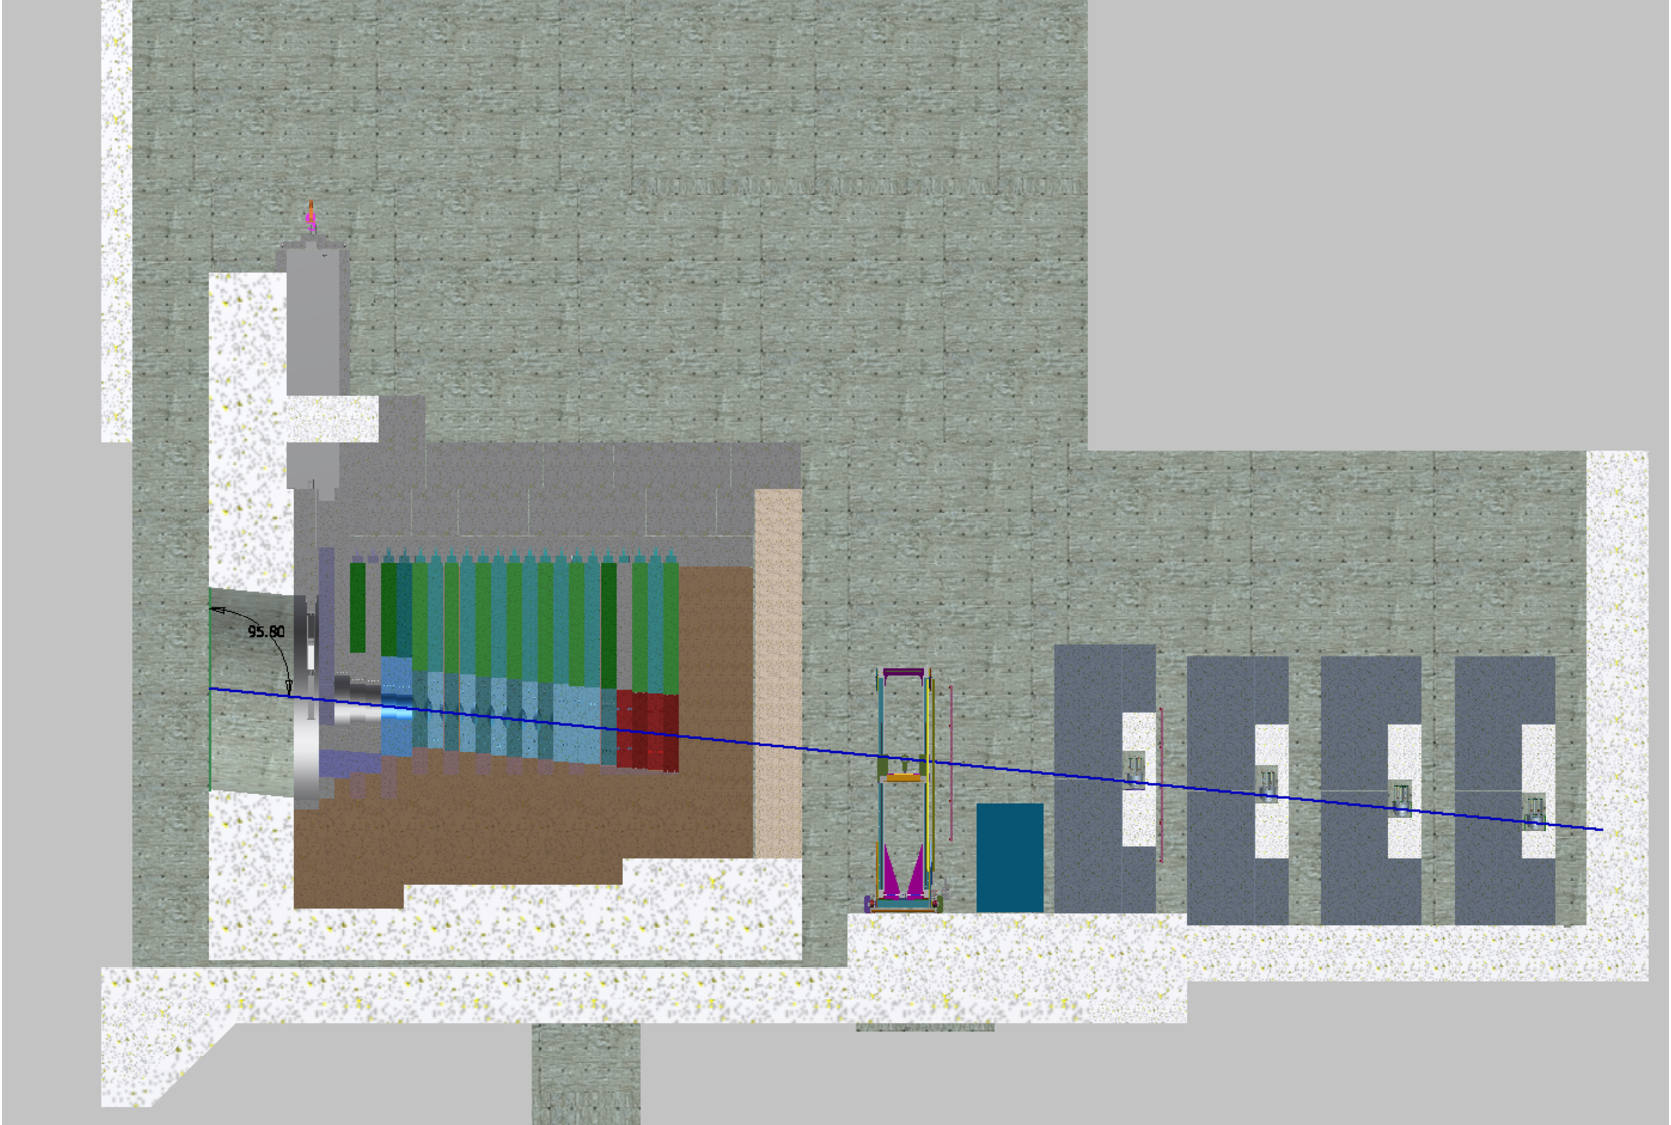
\includegraphics[width=4in,angle=0]{AbsorberElevationView}
\end{cdrfigure}
The absorber itself is encased in
concrete. The first set of muon-measurement devices, from left to
right, is a variable-pressure gas Cherenkov counters, which mounted on
a movable stand in order to scan across the rear surface of the
absorber.  Following that is an array of diamond ionization detectors
and finally a set of stopped-muon counters which are interspersed
between walls of steel ``blue blocks''.  The blue blocks are there to
provide several depths at which to monitor the stopped muons as they
range out in the material. A second array of ionization devices will
also be placed farther downstream within the blue blocks.


Figure~\ref{fig:AbsorberThickness} shows the energy lost by a
horizontal muon as it traverses the absorber, as a function of the
distance from the beam axis along a 45$^\circ$ line perpendicular to the beam axis. 
\begin{cdrfigure}[Energy loss in absorber]{AbsorberThickness}
{The energy loss a muon, parallel to the beam axis, experiences as it traverses 
the material in the absorber. The muon's energy loss is plotted versus the distance 
from the beam axis, along a 45$^\circ$ line perpendicular to the beam axis. Muons 
suffer between 4.7 and 9.3~GeV of energy loss depending upon where they cross the absorber.}
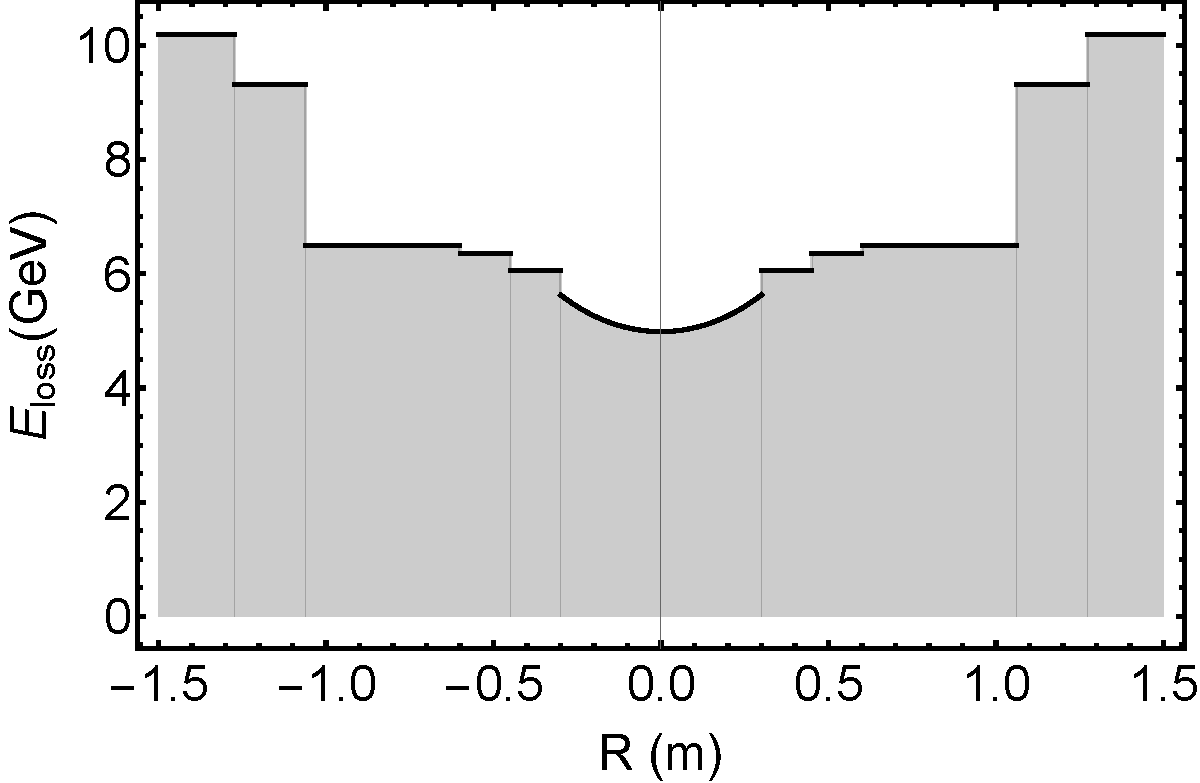
\includegraphics[width=4in,angle=0]{AbsorberThickness}
\end{cdrfigure}
In the central region, roughly to a distance of 105~cm, the muons lose
between 5.0 to 6.4~GeV, so that the lowest-energy muons leaving the
absorber at that point correspond to neutrino energies of $\sim$1.5
to 2.0~GeV. At a radius of roughly 105~cm, the full thickness of steel
causes the muons 10~GeV or more, corresponding to neutrino energies of
$\sim$2.6~GeV. From the perspective of the muon systems it will be
desirable to lower these thresholds if possible.


%
%  REmoved the individual muon component sections per Bill 4/23/15 (AH)
%%%%%%%%%%%%%%%%%%%%%%%%%%%%%%%%%%%%%%%%%%%%%%%%%%%%%%%


\subsection{Installation and Operation}

The muon system detectors, already fully calibrated in the NuMI beam,
will be installed as soon as the absorber hall (LBNF-30) is ready.
Because the system will be located in a radiation-controlled
environment that will not be accessible during beam operation, it is
essential that the electronics and gas handling system be both robust
and remotely operable.  The prototype system in use at the NuMI area
can be relocated for that purpose, or if desired a new system may be
constructed.  Periodic access will be required to the utilities area
to replace gas bottles.

The blue blocks associated with the muon systems will be installed
first.  The positioned stand for the Cherenkov detector system will be
installed next.  and then the various detectors will be installed.
The stopped-muon counters will be placed into the spaces between the
blue-block walls on support frames.  There will be access to the areas
between the shield blocks from the side, and the stopped-muon counters
will be designed so that they can be wheeled in from the side.  If
needed, they could then be moved around to measure the stopped-muon
rates across the muon beam.

The muon systems will be operated continuously in order to insure a
stable, high quality neutrino beam.  The muon-monitor-system data will
be displayed in the control room on a spill-by-spill basis to monitor
the beam stability. Because the system will be located in a
radiation-controlled environment that will not be accessible during
the beam operation, it is essential that the electronics be designed
for remote operation.

\section{Hadron Production Measurements}
\label{sec:detectors-nd-ref-hadron}

\subsection{Introduction}

The technical components that would be needed to implement the
strategies described in this chapter are outside the scope of the DUNE
NDS conceptual design. This information is included in this document
because it complements the conceptual design and expands the NDS
capabilities to more closely meet the mission need without increasing
the project cost.

\subsection{External Hadron-Production Measurements}
\label{sec:detectors-nd-external-hadron}

Uncertainties on hadron production will translate into uncertainties
in the neutrino fluxes in the DUNE Far Detector, since the neutrinos
are produced by hadrons decaying in the decay pipe. Precise
calculations of neutrino fluxes in high-energy accelerator beams are
limited at present by our knowledge of hadron production
cross-sections in hadron-nucleus collisions.  The modeling of
strong-interaction cascades and hadronic yields from ``thick'' targets
(up to a couple of interaction lengths) relies on detailed knowledge
of underlying physics and cross-sections, which must be provided as a
starting point to simulations. The resulting prediction of the flux of
neutrinos, produced from decays of pions, kaons, and muons emerging
from a hadronic shower and beam line re-interactions, is an essential
part of simulations of most neutrino experiments.

Two-detector neutrino oscillation experiments predict the neutrino
flux at the far detector by using neutrino fluxes ``calibrated'' (or
appropriately scaled) by event energy spectra measured in the near
detector. However, these experiments rely on beam simulations since
the decay pipe (where most beam neutrinos are created) provides
different angular acceptance for the two detectors. In addition,
experiments using near and far detectors based on different detection
technologies further complicate the extrapolation. This chapter
outlines the DUNE strategy for augmenting the capabilities of the BLM
with external measurements of secondary-beam particles.
%\fixme{This was originally written when we just had 
%the BLM and no NND; no change needed here? Second point: This sentence should be in the intro paragraph of this chapter.}

\subsection{Background}

A complete knowledge of the momenta and decay points of the kaons, pions and
muons would be sufficient to completely predict the un-oscillated flux of neutrinos
at the Near and Far Detector locations. This would require knowledge of:

\begin{itemize}
\item the phase-space distribution of the initial proton beam
\item details of all materials present in the target, horn and decay pipe areas
\item  the electromagnetic focusing characteristics of the magnetic horn
\item the detailed development of the hadron cascade, spawned by the
initial proton, that passes through the target/horn/decay pipe
\item the meson-to-neutrino decay rates
\end{itemize}

With careful engineering design and careful control of the materials in the target
area, all of these items can be simulated accurately except hadronic cascades in
the target, horn and decay pipe. The simulation of the hadronic cascade requires
accurate knowledge of the hadron scattering cross sections, for which there are no
first-principle calculations. These cross sections must therefore rely on models, which
in turn require hadron-production measurements that span particle type, particle
energy and the various materials found in the target, horn and decay pipe.

At the present time, a sufficient body of hadron-production
measurements does not exist to achieve DUNE's desired accuracy of
4-5\%, as determined by the irreducible error on the statistical
uncertainty for the appearance-measurement background, although this
is expected to improve over time. A program of hadroproduction
measurements has been approved as US-NA61 to run at CERN.
%As the BLM system described in
%Section~\ref{sec:detectors-nd-ref-blm} cannot meet this requirement
%alone, a near-far comparison will be more complicated than in certain
%other neutrino-oscillation experiments, e.g., MINOS
%experiment~\cite{gnumi-validation}.


%\subsection{The US-NA61/SHINE Program}
%\label{sec:detectors-nd-blm-external-usna61}
%
%A proposal to make measurements for the Fermilab neutron program with the NA61/SHINE experiment has been funded by DOE/HEP \cite{ref:NA61Proposal,ref:NA61Addendum} , US-NA61, and recommended by the CERN SPSC. NA61/SHINE is situated in the North Area of CERN on the H2 beam line. 
%
%The detector, schematically shown in Figure~\ref{fig:NA61Scheme} is comprised of two large air gap, Helmholtz-coil superconducting magnets with a total bending power of 9 T-m. The detector is instrumented with gas TPC tracking, time-of-flight counters, and a hadron calorimeter (at very forward angles). The US-NA61 measurements will provide hadron-production data sufficient for predicting neutrino fluxes at DUNE. A pilot run of 120~GeV/c protons interacting on a thin 4\% graphite target was taken by NA61 during July, 2012. A 4-week dedicated physics run is scheduled for October, 2015.
%
%The run plan for the 2015 data is shown in the table in Figure~\ref{fig:NA61RunPlan}. The initial run will focus on proton and pion data at 120 GeV/c and 60 GeV/c energies. This will constrain well extrapolations from higher and lower energies that are currently under use in neutrino beam simulations.
%
%\begin{cdrfigure}[A schematic drawing of the CERN NA61 detector]{NA61Scheme}{A schematic drawing of the CERN NA61 detector, a hadron production and heavy ion experiment designed to measure hadrons over a large part of the relevant phase for neutrino experiments. The TPCs, shown in blue, can separate pions from protons and kaons.}
%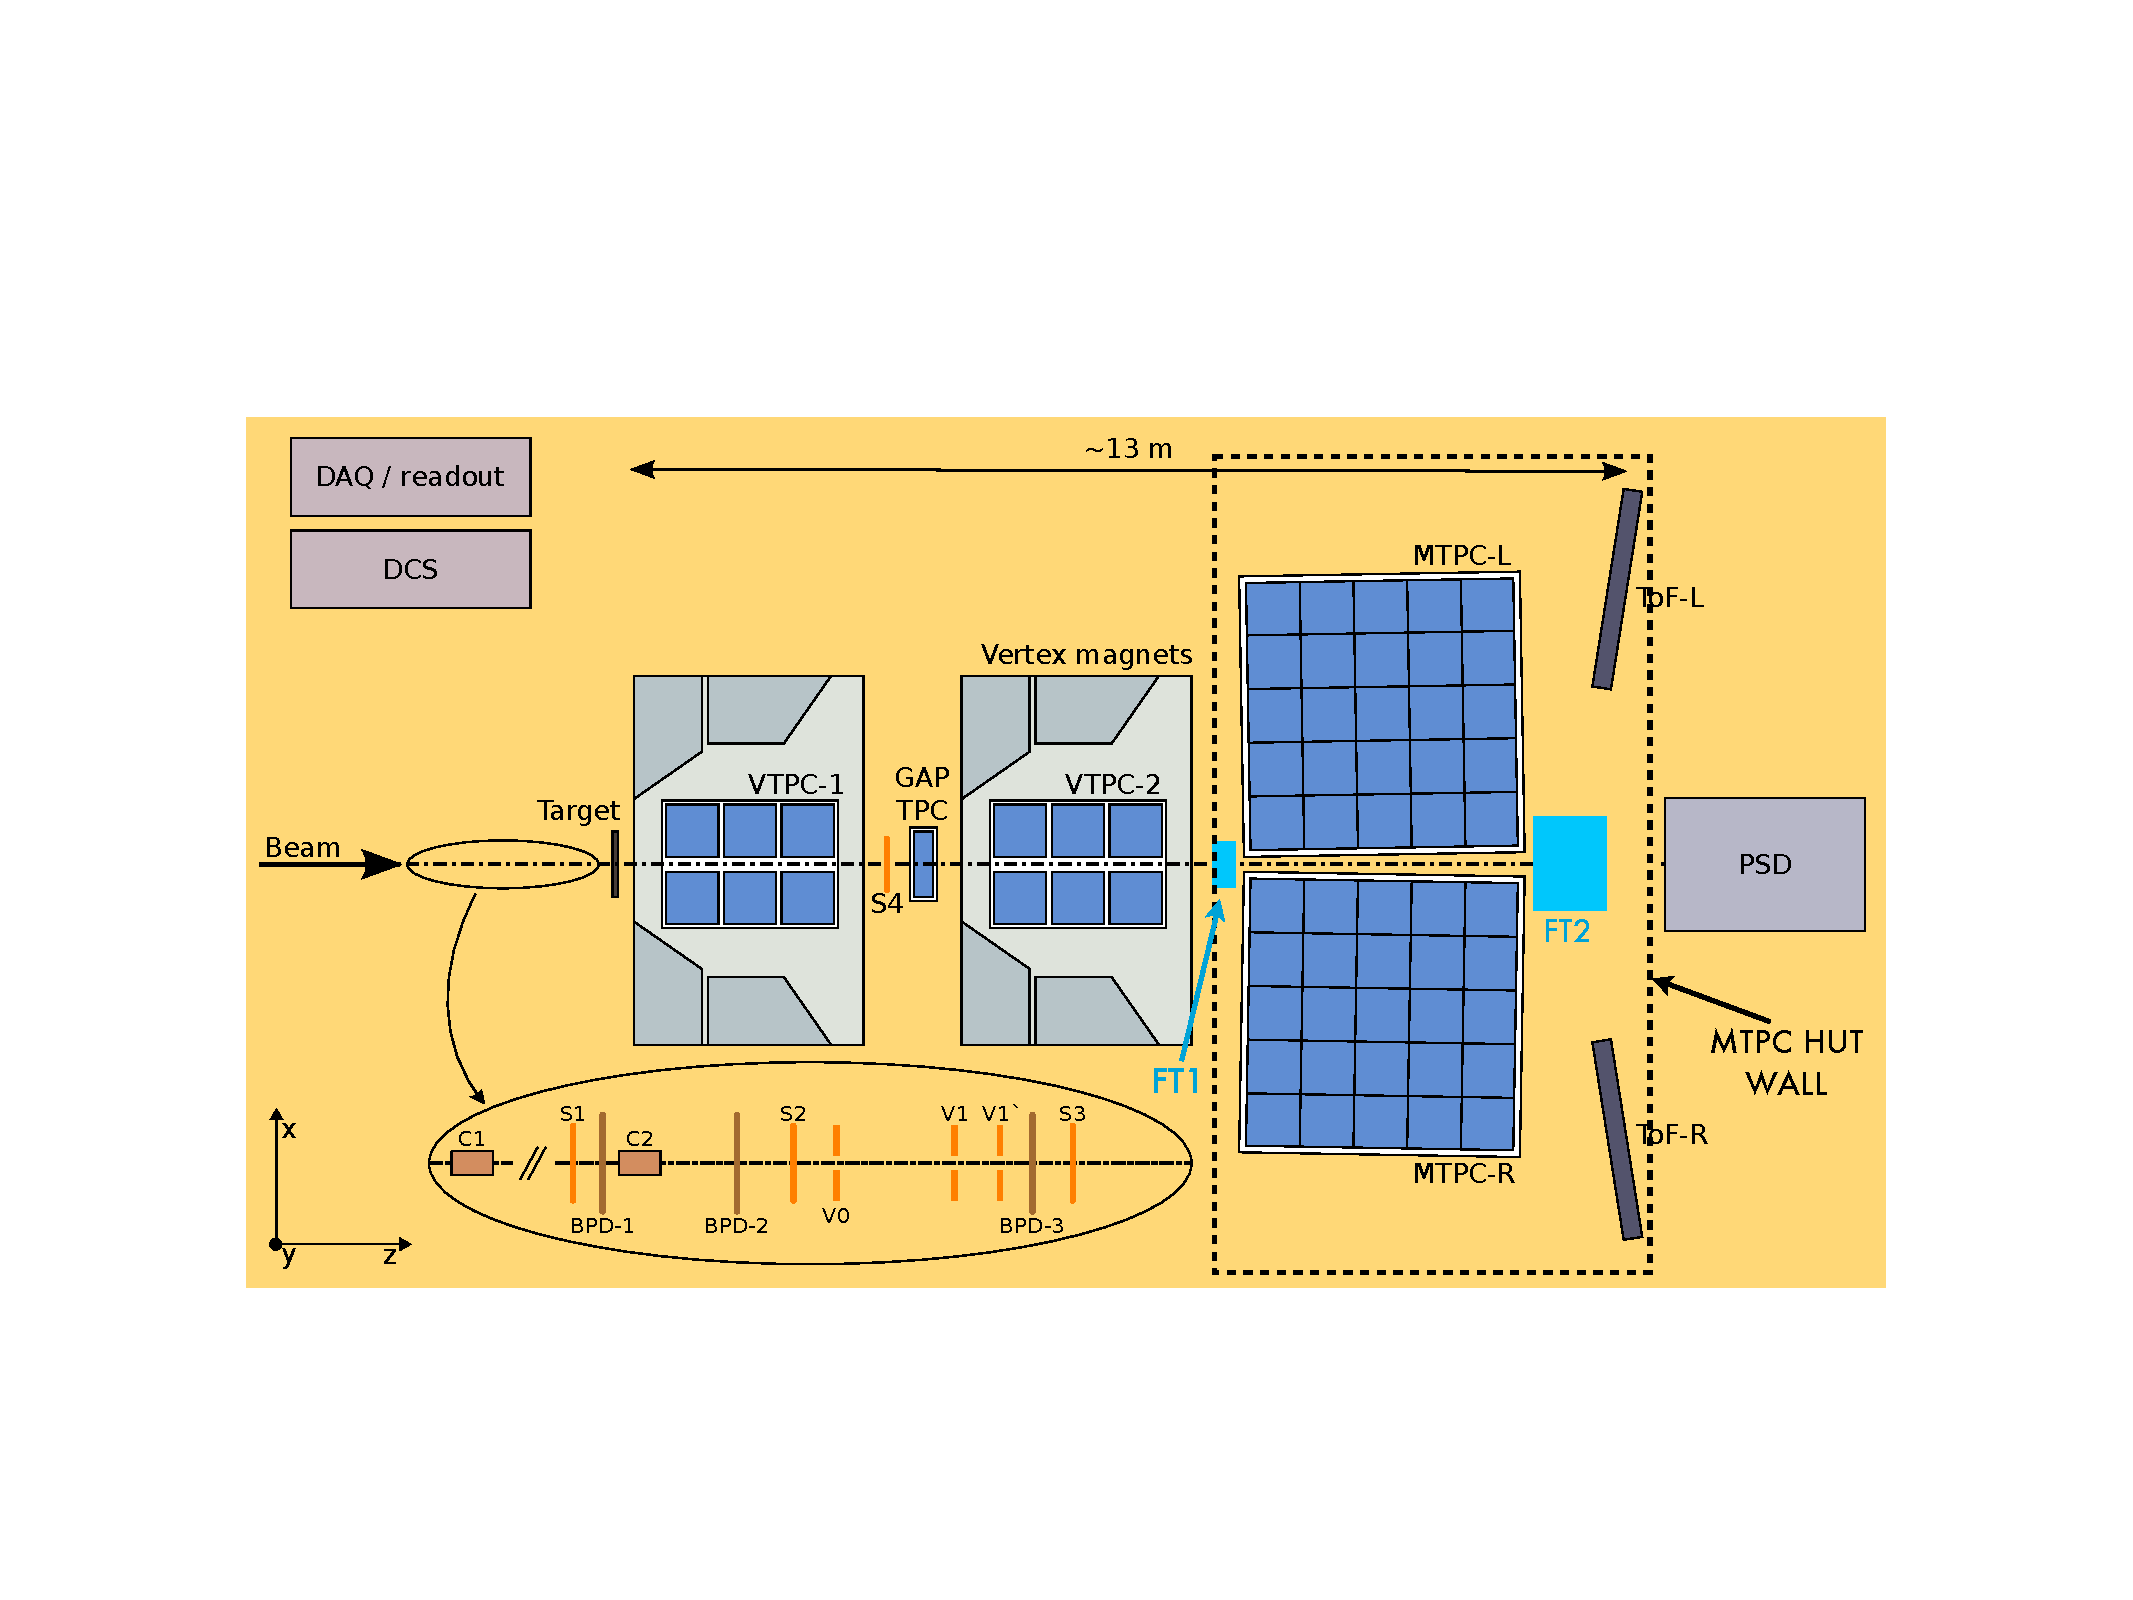
\includegraphics[width=4in]{NA61-PlanView}
%\end{cdrfigure}
%
%\begin{cdrfigure}[The 2015 run plan for US-NA61.]{NA61RunPlan}{A table that shows the proposed run plan for 
%the US-NA61 data run in the fall of 2015.}
%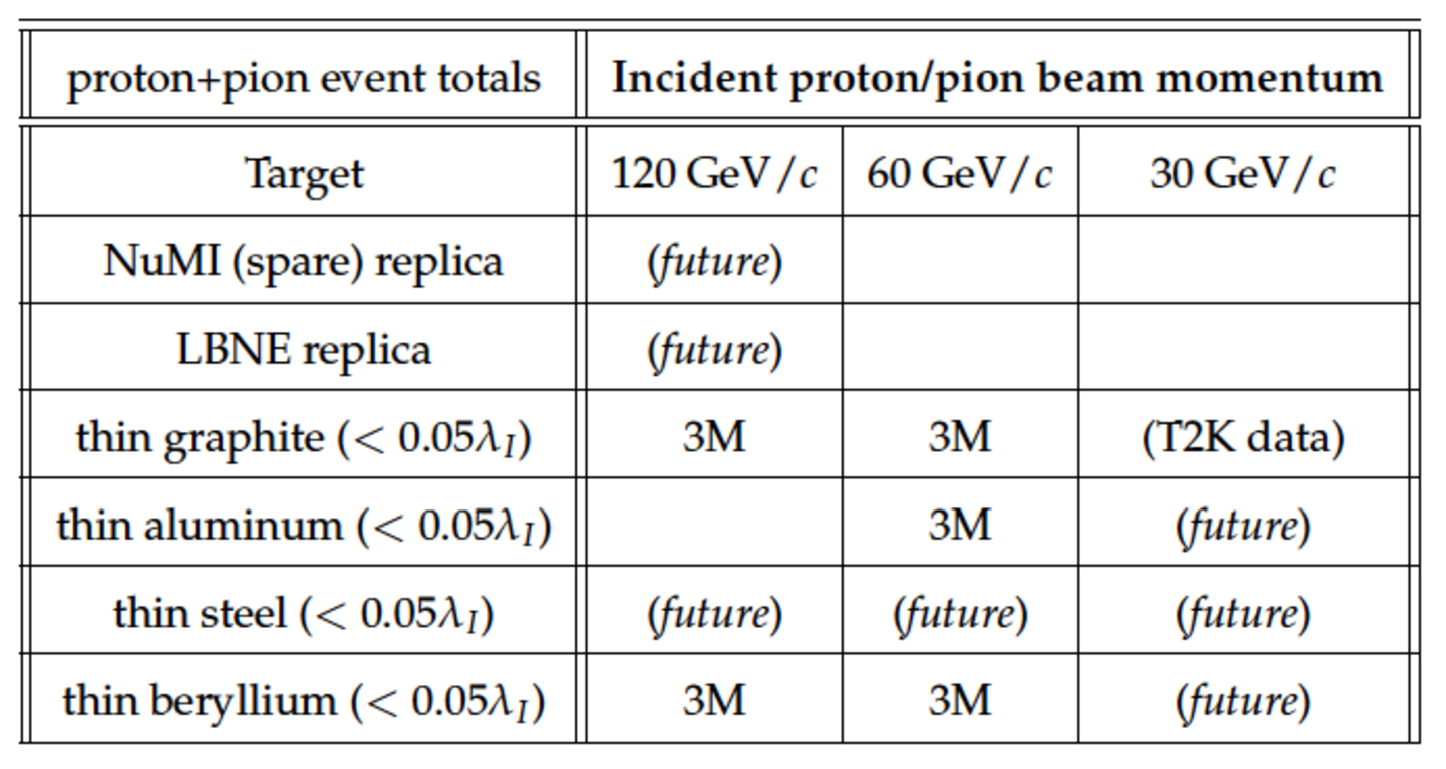
\includegraphics[width=4in]{NA61RunPlan}
%\end{cdrfigure}

